\subsection{Sensitivity Analysis Without Front-end Processors}
\subsubsection{Data Injection on The Corner Processor}
The simulation result of sensitivity analysis of $2*n$ regular network \Fig{2t10} is as follows:
\begin{figure}[!ht]
\centering
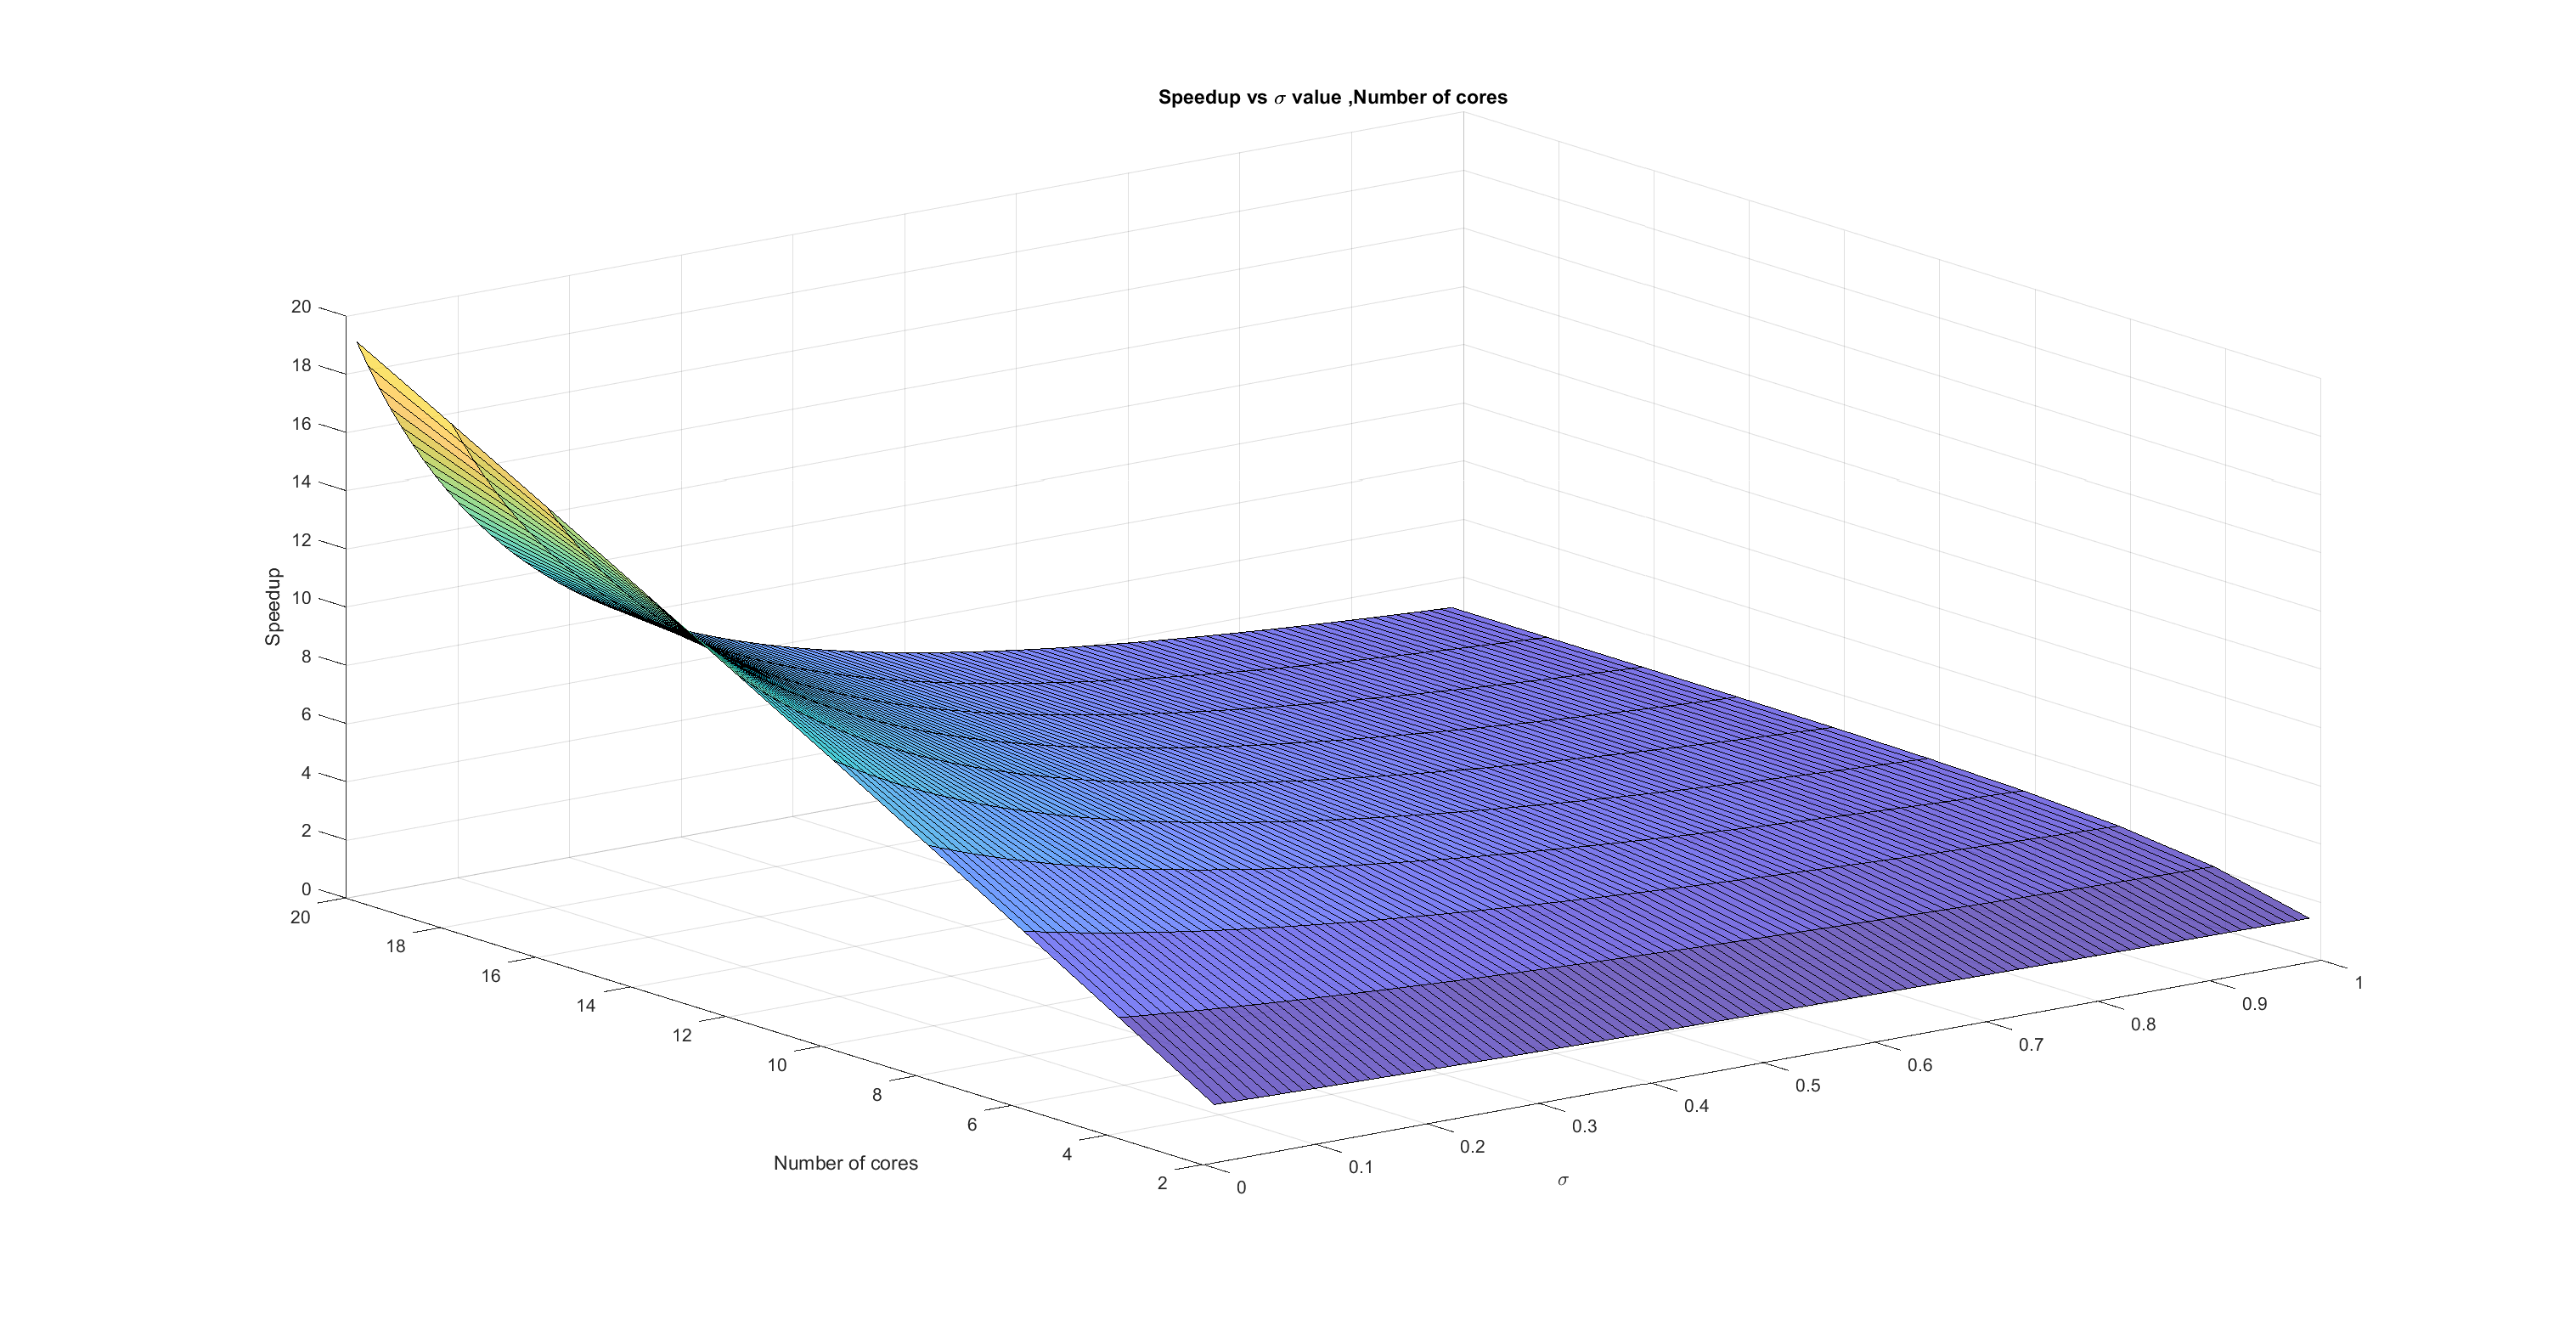
\includegraphics[width=1\columnwidth]{figure/sa2t10c_no.eps}
\caption{Sensitivity analysis result of 2*10 regular network result}
\label{fig:sa2t10c_no}
\end{figure}

The figure illustrates that if $\sigma < 0.  1$, the number of cores grow up, the speedup efficiency is likely linear increasing.   Alternatively speaking, if $\sigma < 0.  1$, the number of cores dominate the efficiency.   If the $\sigma > 0.  2$, the efficiency drops dramatically.   That is, the $\sigma$ value plays more critical role in the speedup simulation.   This important investigation benefit the multi-source assignment problem.   In addition, if the number of cores is bigger than $4$, the bottom speedup effect is about $3$ time.   
\newpage

\subsubsection{Data Injection on The Boundary Processor}
\begin{figure}[!ht]
\centering
\includegraphics[width=1\columnwidth]{figure/sa3t8b_no.eps}
\caption{Sensitivity analysis result of 3*8 regular network result}
\label{fig:sa3t8b_no}
\end{figure}

\Fig{sa3t8b_no} tells the simulation result for the data injection on the boundary.  

\newpage 
\subsubsection{Data Injection on The Inner Grid Processor}
\begin{figure}[!ht]
\centering
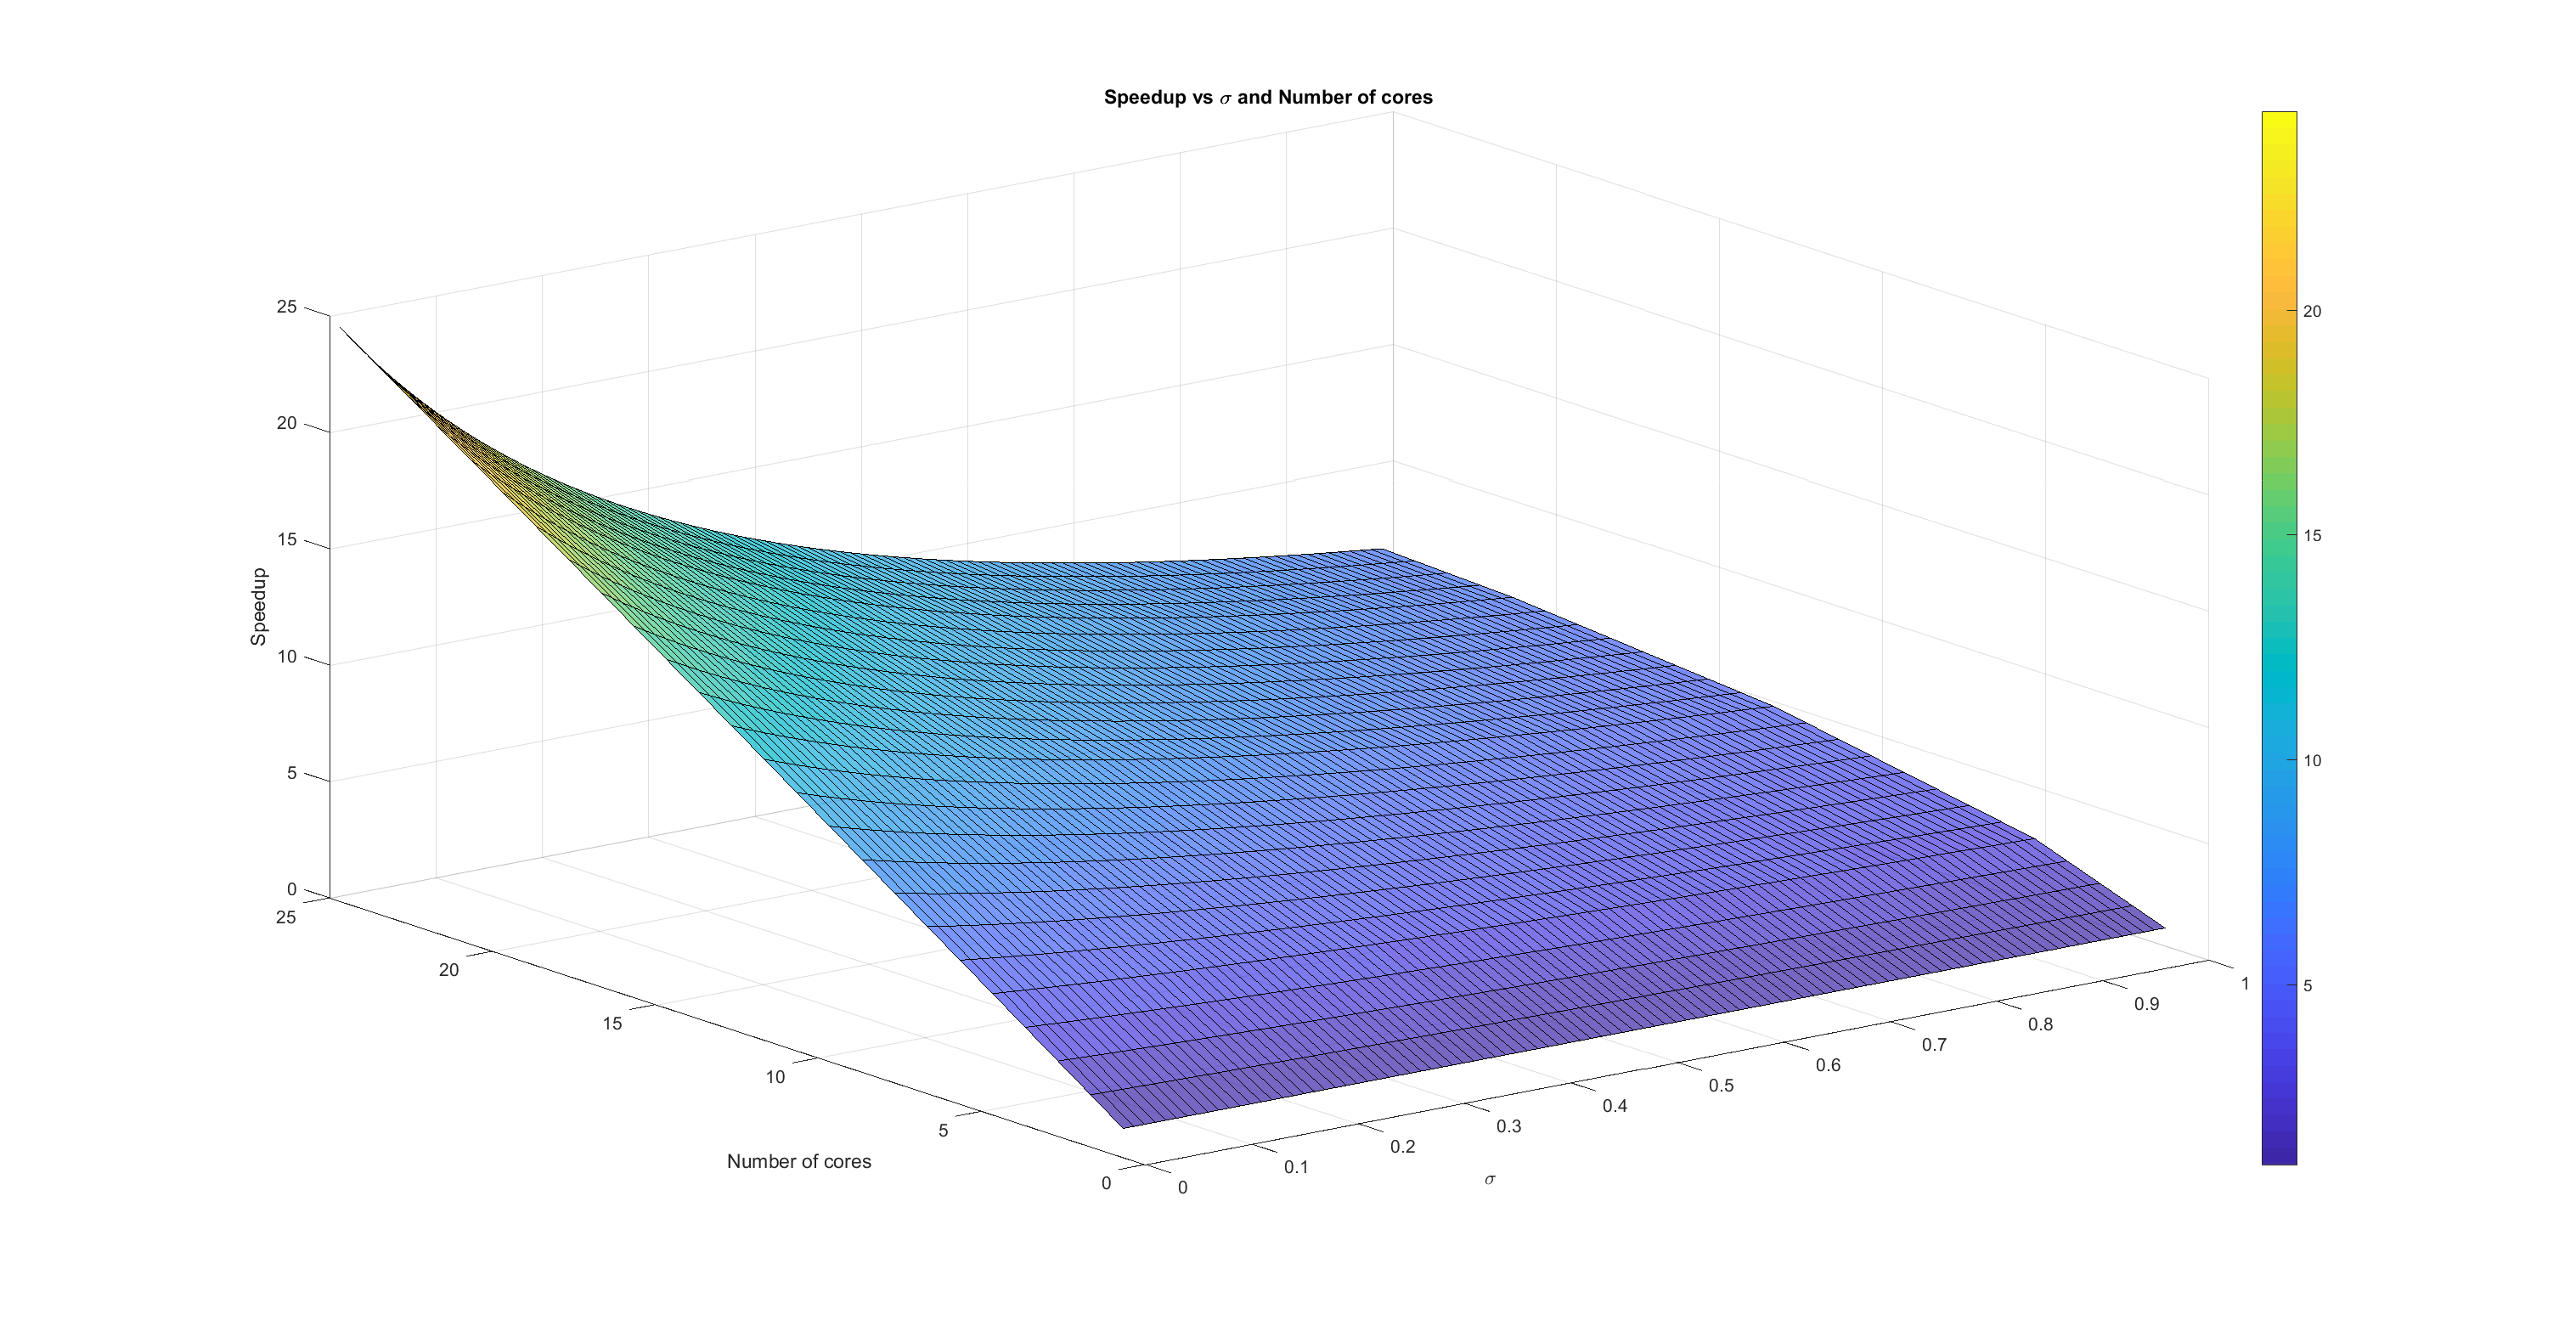
\includegraphics[width=1\columnwidth]{figure/sa5t5i_no.eps}
\caption{Sensitivity analysis result of data injection position on inner grid processor}
\label{fig:sa5t5i_no}
\end{figure}

\Fig{sa5t5i_no} displays the simulation result for the data injection position $P_{12}$.   If $\sigma < 0.1$, the speedup linear grows up and the best speedup is $24$, which happens on the $\sigma < 0.1$.   